\chapter{iBeacon} \label{chap:ibeacons}
At Apple's yearly \ac{WWDC} 2013 Apple introduced a new technology, called \emph{iBeacon}, to enhance smartphone applications' location awareness.

An iBeacon, in general a beacon, is a System-on-Chip which emits a \emph{\acf{BLE}} signal in a predefined time interval, analogous to a lighthouse. Devices with compatible hardware and software, for example iPhone\,4\,S and Android version~4.3 and later versions, can receive the signals, to provide the user location based services. Typically, a beacon's size is less the size of a child's hand, and is powered by a small battery to be independent from its environment. Thus, it easily can be attached to another object to establish a region around the object. A smartphone app can then provide the user with a notification, once the user enters or leaves the region, by estimating the proximity to the beacon \citep{apple:getting_started,binside:ds}. According to \citet{binside:ds}, typical use-cases are:
\begin{itemize}
  \item Location based marketing (e.g.\ digital coupons and digital signage of articles)
  \item Proximity sensing to an object
  \item Indoor localization and navigation (e.g.\ digital museum guide and airport guide)
\end{itemize}

\noindent After providing a brief idea what a beacon actually is, the next sections focuses on the communication technology which is used by a beacon to send its signal and the beacons itself. Afterwards, the \acs{API} provided by Apple's mobile operating system iOS~8.1 to receive these signals is described. After providing the basics, the evaluation results from the proximity estimation to a beacon are presented. This results are important for the algorithm's implementation as described in Chapter~\ref{chap:pf}.


\section{Bluetooth Low Energy}\label{sec:ble}
\ac{BT} is a wireless short range communication technology with the intent to replace, or reduce the amount of required cables. It is developed by the \emph{Bluetooth Special Interest Group (Bluetooth SIG)} which is a large group of companies, such as chip manufacturers. The technology's key features are robustness, low cost and low power consumption. It is often used to connect a car's speaker phone with a smartphone, to connect a wireless keyboard or mouse with a computer, or to exchange files between two cell- or smartphones.

Originally, the \acl{BT} specification contained just one wireless technology system called \emph{\ac{BR}/\ac{EDR}}. Since version~4.0, released in 2010, the specification adds a second technology named \emph{\ac{LE}}. The term \ac{LE} is the technology's name as described within the specification. The technology's official (marketing) label is \emph{Bluetooth Smart}. Devices labeled with it are only equipped with the \ac{LE} technology. In contrast, devices labeled with \emph{Bluetooth Smart Ready} are equipped with both technologies, the traditional \ac{BR} and the \ac{LE} technology \citep{bluetooth:spec}. One of the differences is speed. \ac{BR}/\ac{EDR} has a max.\ transfer rate of 2-3~Mbps; whereas, \ac{LE} is designed only for 1~Mbps. But, \ac{LE} has the advantage of having a low current consumption. Its complexity is also lower than the one of \ac{BR}/\ac{EDR} \citep{bluetooth:spec}.

Usually iBeacons are Bluetooth Smart devices \citep{binside:ds}. To get a better idea of how the communication between a smartphone and an iBeacon works, the following sections provides an overview of the \ac{BLE} technology.


\subsection*{Channels and Events}
Both \ac{BT} systems use the 2.4GHz frequency band. \ac{BLE} divides the band into 40 channels. Three of them are advertisement channels, the others are data channels. These channels are used to transmit events, which consist of typical data packages. The \ac{BLE} specification distinguishes between two event types, the \emph{advertisement} and the \emph{connection} event.

Advertisement events are used for unidirectional or broadcast communication between two or more devices. In addition \emph{connectable advertisement} events to establish a pair-wise or bidirectional communication do exist. Advertisement events are transmitted via one of the advertisement channels. The device which sends the advertisement is called the \emph{advertiser}. The device looking for these events is called \emph{scanner}.

If a device looks for a \emph{connectable advertisement} to establish a connection, it is called the \emph{initiator}. It becomes the \emph{master} after establishing the connection. The advertising device becomes the \emph{slave}. Master and slave(s) form a piconet. Slaves in a piconet cannot communicate with each other. The connection establishment takes place on one of the advertisement channels. After establishing a connection, the communication takes place on the data channels by using frequency hopping instead of one specific channel \citep{bluetooth:spec}.

\subsection*{Operations}
According to \citet{bluetooth:spec}, \ac{BLE} implements different operations for the above mentioned event behavior:
\begin{itemize}
  \item To send advertisement events the \emph{Advertisement Procedure} is used. It sends unidirectional broadcast messages without a connection to other devices. If the device itself is already connected to another device, it can only send non-connectable advertisements. Advertisements can contain user data. A scanner can respond to an advertisement to request more user data.
  \item The \emph{Scanning Procedure} must be used to listen for advertisement packages. It can read the user data sent in an advertisement. Scanning is possible while being connected to a device.
  \item It is possible to listen just for a specific set of devices. In order to do that the \emph{Device Filtering Procedure} needs to be used.
  \item The \emph{Discovering Procedure} can be used to look for specific devices. It  uses device filtering.
  \item To establish a connection the \emph{Connecting Procedure} must be used.
  \item After the connection establishment the \emph{Connected Procedure} is used to transfer data.
\end{itemize}

\subsection*{Security}
As mentioned by \citet{bluetooth:spec}, the data is encrypted by the \emph{AES-CCM} encryption method. For authentication it provides three different modes for different device capabilities:
\begin{itemize}
  \item \emph{Just Works}: Requires just a possibility to tell the device, that it should accept a connection request of an unknown device. A hardware button can be used, that the user needs to press for a few seconds for the initial connection establishment. The method is often used if the slave has no possibility to enter a key, e.g.\ to connect a smartphone with a bluetooth headset.
  \item \emph{Passkey Entry}: Requires the input of a PIN code. Here, the master needs the possibility to show a PIN code and the slave needs some sort of keyboard. A typical example is the pairing process of a \ac{BT} keyboard with a computer. The computer displays a code and the user has to enter it on the keyboard that wants to connect.
  \item \emph{Out of Band}: Requires a separate channel which is used for the discovery and also for the exchange of the secure key; for instance, a wired connection.
\end{itemize}


\subsection*{Adverting and Response Data}
Besides the mentioned user data, the advertisement and response always contain data such as the \emph{local name} of the device, which can be used to identify it, information about the \emph{manufacturer}, and the \emph{\acs{TX}-power level}, which was used to send the data packages. Furthermore, it includes \emph{flags} which provide information whether the device is in limited discoverable mode, if the device supports also \ac{BR}/\ac{EDR}, if both modes can be used simultaneously, and further service-specific data.


\subsection*{Summary}
\acl{BLE} is a separate wireless communication technology which was added to the traditional \acl{BT} system. Devices equipped with a \ac{BT} chip of version~4, can either support both systems or just one. \ac{BLE} is low cost and has low power consumption. Thus, it is possible to produce cheap devices like iBeacons which can be powered over months with a coin cell.

Often, the question comes up, whether beacons can be used to track users, i.e.\ their smartphones. To do so, a response from the smartphone must be sent. As shown, advertisements do not require a response; thus, tracking would only be possible by establishing, or at least trying to establish, a connection. But due to the fact, that just one connection at the same time can be established, and thus a device can only talk to one beacon, connection establishment cannot take place. Consequently, the claim made by \citet{apple:getting_started}, that tracking or putting ``user's private data at risk'' is not possible, is true.

\section{Beacon}\label{sec:beacon}
As mentioned before beacons are small System-on-Chip devices, which send \acs{BLE} signals. To manufacture beacons, compatible with Apple's iBeacon standard, or to get an insight in the official specification, a license from Apple needs be obtained. Thus, I am focusing on the publicly available documentation, which describes the relevant parts with enough detail for the purpose of this thesis.

This section provides first an insight into the generally valid details. Afterwards, the possible configuration parameters of the beacons' hardware are outlined. Finally, the necessary steps for the beacon deployment are described.

\subsection{General Details}
In general, each beacon sends a \acs{BLE} signal in a fixed time interval. On one hand, the signal contains information to uniquely identify a beacon, and on the other hand, data to be able to estimate the proximity, i.e.\ the distance, between the beacon and the device itself.

\subsubsection*{Identifier}
The unique identifier consists of three parts, the \texttt{proximityUUID}, \texttt{major}, and \texttt{minor}, which together form a unique identifier. Usually, a smartphone's application is not interested in all beacons that are around, but rather in a specific subset. Thus, the application has to ``tell'' the \ac{OS} in which it is interested in. The intention of the identifier's three parts is to build a hierarchical identifier system for beacons, to be able to search for a subset. The following example explains the three parts and their purposes:

Imagine a chain of stores' application which needs to support several shops. Each shop has multiple beacons deployed. Thus, the application is only interested in beacons belonging to the chain of stores. Furthermore, the application needs to know in which shop the user is located, or even in front of which beacon.

\begin{itemize}
  \item \textbf{\texttt{proximityUUID}} (16 bytes): All beacons that belong to the same cain of stores share the same \acl{UUID}. Thus, the application can just search for this part of the identifier, i.e.\ for being notified once the \ac{OS} receives any beacon signal belonging to the chain of stores.
  \item \textbf{\texttt{major}} (2 bytes): All beacons deployed in the same shop share the same \texttt{major} identifier. Consequently, the app is able to differentiate between shops. Furthermore, it can just search for beacons of a specific shop without having a lot of overhead.
  \item \textbf{\texttt{minor}} (2 bytes): Each beacon in a shop has a different \texttt{minor} identifier. Hence, by combining all three identifiers, the app can determine in front of which beacon in a certain shop the user is located.
\end{itemize}

\noindent Typically, these three parts can either be configured on the beacon itself, if not they need to be manufactured with the desired identifiers \citep{apple:getting_started,binside:ds}.

\subsubsection*{Proximity estimation}
As mentioned in Chapter~\ref{chap:fundamentals}, there are several physical methods to estimate the distance between a transmitter of a radio frequency signal and the receiver. In this case the \acf{RSS} is used to estimate the proximity. Consequently, the receiver needs to know which \acs{TX}-power level is used to send the radio frequency signal. As mentioned in Section~\ref{sec:ble}, \ac{BLE}, uses the 2.4~GHz frequency. According to \citet{apple:getting_started} and \citet{binside:ds}, signals of this frequency band are heavily attenuated in obstructed environments and especially by water. Consequently, the knowledge of the sender's \acs{TX}-power level is not sufficient to estimate the distance. Thus, a calibration value, which is the \acl{RSS} in a distance of 1m, is also sent to the receiver. Therefore, the later described calibration step, after deploying the beacons is necessary.

\subsection{Hardware Specification}
To test and evaluate the implementation I used ten beacons from a company called \emph{BEACONinside GmbH} from Berlin, Germany. The beacons have the Model No.: B0001-A (HW: Rev 1.1, SW: 1.0). Figure~\ref{fig:bi:beacons} shows a 3D picture of sections of the beacons. According to \citet{binside:ds}, the beacons' signal have a range from 0 up to 40 meters. The chipset they used was manufactured by Texas Instruments (Model CC2541). The company obtained a license from Apple to manufacture the beacons, which are compatible to Apple's iBeacon specification~\citep{binside:ds}.

\begin{figure}
	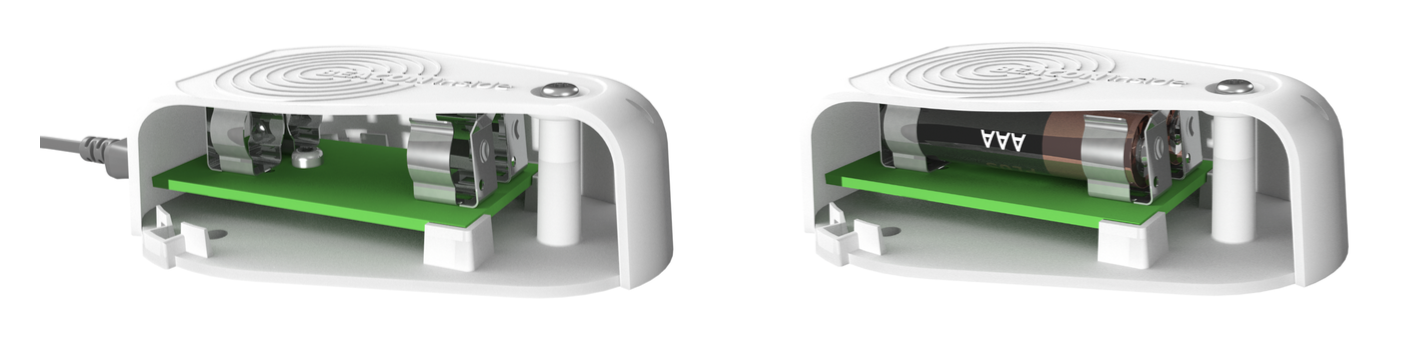
\includegraphics[width=0.6\textwidth]{figures/BEACONinside_beacons}
	\caption{A 3D picture of sectioned beacons \citep{binside:ds}.}
	\label{fig:bi:beacons}
\end{figure}

The beacons's size is 5.8\,cm\,$\times$\,7.96\,cm\,$\times$\,2.25\,cm. They can either be powered by two AAA~batteries to provide a lifespan of approximately one year, or by an external power supply over micro-USB~\citep{binside:ds}.

The beacons are configurable with standard \ac{BLE} tools, like compatible smartphone apps. Such an app establishes a \ac{BLE} connection to the beacon. Each of the following configurable values can be accessed with a specific key. To configure the beacons an iOS app called \emph{LightBlue --- Bluetooth Low Energy}\footnote{Link to the LightBlue App in the iOS AppStore (last access: 23.04.2015) \url{https://itunes.apple.com/de/app/lightblue-bluetooth-low-energy/id557428110}} from a company named \emph{Punch Through Design LLC.}, recommended by BEACONinside is used. According to \citet{binside:ds}, the following values are configurable:
\begin{itemize}
  \item \textbf{\texttt{proximityUUID}:} For instance \texttt{F0018B9B-7509-4C31-A905-1A27D39C003C}
  \item \textbf{\texttt{major}:} A value between 1\,--\,65535
  \item \textbf{\texttt{minor}:} A value between 1\,--\,65535
  \item \textbf{\texttt{\acs{TX}-power level}:} It defines the power level which is used to transmit the beacons advertisement packages, i.e.\ the signals. It can either be 0\,dBm (default) which is the maximum power level, -6\,dBm or -23\,dBm which is the minimum power level.
  \item \textbf{\texttt{Advertising interval}:} Defines the time interval (100\,ms\,--\,10\,s) in which advertisements are sent. The default time interval is 400\,ms, configurable in steps of 625\,$\mu$s.
  \item \textbf{\texttt{Calibration value}:} To estimate the distance of the receiving device to the beacon a calibration step is necessary. The measured \acs{RSS} in a distance of 1m needs to be sent by the beacon with every advertisement. This value can be configured for each \texttt{Tx-power level}. The default is 65\,dBm for the 0dBm power level. It needs to be encoded as the 2' complement in hexadecimal (e.g.\ 65\,dBm = \text{0xBF}).
  \item \textbf{\texttt{Passkey}:} To set one of this configuration parameters the (6 digit) passkey must be entered. The beacons' default value is \texttt{555555}.
\end{itemize}

\noindent Additionally, the following read-only properties about the device and its state are provided~\citep{binside:ds}:
\begin{itemize}
  \item \textbf{\texttt{Device Name}:} The beacon's name consisting of \texttt{BEACON} and the latter three bytes of its \acs{MAC} address.
  \item \textbf{\texttt{Model Number}}
  \item \textbf{\texttt{Serial Number}}
  \item \textbf{\texttt{Hardware Revision Number}}
  \item \textbf{\texttt{Software Revision Number}}
  \item \textbf{\texttt{Manufacturer Name}}
  \item \textbf{\texttt{Battery Level}:} The battery power level in percent.
  \item \textbf{\texttt{Temperature}:} The hardware's temperature in degrees Celsius.
\end{itemize}

\noindent To load the new values after changing the beacon's configuration, the beacon needs to be rebooted. The beacon can also be reset to factory defaults~\citep{binside:ds}.

\subsection{Deployment and Calibration}
As mentioned before, the \ac{BLE} signal quality is heavily influenced by physical materials due to the fact that \ac{BLE} uses the 2.4\,GHz frequency. Especially, water which is a main part of the human body, attenuates the signal~\citep{apple:getting_started}. Thus, the beacons need to be carefully deployed. Ideally, they should be deployed in a manner, that most often the line between beacon and receiver is unobstructed. There should also be enough space around the beacon, that its signal can spread out. By deploying them carefully, the signal's attenuation and other effects like multi-path fading and shadowing can be reduced~\citep{apple:getting_started,IEEE:survey_wireless_indoor_pos}.

The next step is the calibration step. To be able to estimate the distance between smartphone and beacon a reference value is needed. The reference value, as mentioned before, is the measured \ac{RSS} in a distance of 1m to the beacon. The calibration value is configured on the beacon itself, which includes it in the sent advertisement together with its identifier.

According to \citet{apple:getting_started}, the smartphone needs to be positioned in 1m distance to the beacon in portrait mode with the device's top half uncovered. Then the \ac{RSSI} values were collected for at least 10\,s. Meanwhile, the user should slowly move the device on an $\approx$\,30\,cm line in front of the beacon, by maintaining distance and orientation. After collecting the values, the average value is calculated and configured on the beacon. It is advisable, to double check the device's estimated distance, after setting the calibration value. Due to the above mentioned problems, this needs to be repeated for every single beacon.

\section{API --- iOS 8.1}
After describing what beacons are and how they work, this section focuses on the receivers side, especially on the \acs{API} provided by Apple's iOS~8.1 platform. The \acf{CL} framework's \texttt{CLLocationManager} component provides two functionalities, called \emph{region monitoring} and \emph{beacon ranging} to receive a beacon's signals within an iOS app \citep{apple:ios_doc_cl}.

\subsection*{Region monitoring}
As the name already implies, the operating system monitors a specified region and notifies the application, when the user entered or left the region. This functionality is not restricted to regions established by beacons. It already existed long before, and monitors circular regions specified by a distance around a global position in longitude and latitude, e.g.\ a \acs{GPS} position.
iOS monitors the specified regions also if the application is in background mode or is currently not running. If the user enters or leaves a region, the application is launched by the \ac{OS}; for instance, to display a notification to the user \citep{apple:wwdc_2012_bruins,apple:wwdc_2013_bruins,apple:ios_doc_cl}.

\subsection*{Proximity to a Beacon}
To continuously estimate the proximity to a beacon, \emph{beacon ranging} must be used. To use this a \texttt{CLBeaconRegion} needs to be specified. The \texttt{CLBeaconRegion} object requires at least the beacon's \texttt{proximityUUID}. Furthermore, it is possible to specify a specific set of beacons, by adding the beacons' \texttt{major} identifier. Of course they have to share the same major identifier. By additionally providing a \texttt{minor} identifier, the framework searches only for one specific beacon~\citep{apple:wwdc_2013_bruins,apple:ios_doc_cl}.

After starting the search, the \texttt{CLLocationManager} starts to notify the before specified \texttt{delegate} object in a continuous manner after it received the first advertisement from a beacon, which it is supposed to look for. This means that the \texttt{CLLocationManager} does not call the \texttt{delegate} until it receives the first matching beacon advertisement. After the first call it continuously calls the delegate approximately every second regardless of whether it actually received a beacon's advertisement or not.

The \texttt{CLLocationManager} passes an array of \texttt{CLBeacon} objects to its delegate. Each of it represents one beacon. Table~\ref{tab:beaconExampleData} shows two example data sets, which the \texttt{CLLocation\-Manager} passes to its delegate. Each data set contains four \texttt{CLBeacon} objects. The table's last entry represents a beacon, which is out of range.

\begin{table}
	\begin{tabular}{*{7}{c}}
time & proximityUUID & major & minor & proximity & accuracy & rssi \\
\hline
1.0400 & F0018B9B-\dots-1A27D39C003C & 21500 & 48945 & 2 & 1.2915 & -67\\
1.0400 & F0018B9B-\dots-1A27D39C003C & 39821 & 56686 & 2 & 5.9948 & -79\\
1.0400 & F0018B9B-\dots-1A27D39C003C & 41738 & 1201 & 3 & 6.8129 & -80\\
1.0400 & F0018B9B-\dots-1A27D39C003C & 38722 & 6270 & 3 & 7.7426 & -81\\
 & & & & & & \\
2.0387 & F0018B9B-\dots-1A27D39C003C & 21500 & 48945 & 2 & 1.4452 & -68\\
2.0387 & F0018B9B-\dots-1A27D39C003C & 39821 & 56686 & 3 & 5.5235 & -78\\
2.0387 & F0018B9B-\dots-1A27D39C003C & 41738 & 31201 & 3 & 6.8129 & -80\\
2.0387 & F0018B9B-\dots-1A27D39C003C & 38722 & 6270 & 0 & -1 & 0\\
\end{tabular}

	\caption{Two successive example datasets of \texttt{CLBeacon} objects passed by the \texttt{CLLocationManager} to the specified delegate. The column \emph{time} shows a relative timestamp, to simplify the table.}
	\label{tab:beaconExampleData}
\end{table}

A \texttt{CLBeacon} object contains on one hand the beacon's identifiers, as described in Section~\ref{sec:beacon}. On the other hand, it contains three values, which express the beacons proximity in different ways.

\subsubsection*{\acs{RSSI} Property}
The \texttt{rssi} property, stores the \acl{RSS} measured in dBm. It expresses how strong the received signal is. As mentioned before, a beacons' advertisement time interval can be specified. Remember, the used beacons send their advertisement per default every 400ms. The framework itself sticks to its $\approx$\,1\,s time interval. It collects all received advertisements and calculates the average since the last reported \texttt{rssi} value. If a beacon's signal was received before, but not during the current time interval, its \texttt{rssi} value is 0 \citep{apple:wwdc_2013_bruins,apple:ios_doc_cl}.

\subsubsection*{Proximity Property}
The \texttt{proximity} property's value expresses the relative distance to a beacon. It can either be \texttt{unknown\,=\,0}, \texttt{immediate\,=\,1}, \texttt{near\,=\,2}, or \texttt{far\,=\,3}. The \texttt{unknown} state means, that the proximity could not be detected. One reason could be, that the \emph{beacon ranging} just started but not enough advertisements were received. The \texttt{immediate} state ``represents a high level of confidence that the device is physically very close to the beacon''~\citep{apple:getting_started}. The \texttt{near} state is reported, if the user is in approximately 1\,--\,3\,m proximity to the beacon. Consequently, the \texttt{immediate} state is reported if the user is closer than $\approx$\,1\,m and the state \texttt{far} is reported if the ``beacon device can be detected but the confidence in the accuracy is too low to determine either Near or Immediate''~\citep{apple:getting_started}. Hence, the estimated distance is larger than $\approx$\,3\,m.

\subsubsection*{Accuracy Property}
The object's \texttt{accuracy} property actually expresses the proximity to a beacon in meters, but \citet{apple:ios_doc_cl} describes the property as follows:
\begin{quote}
  ``The accuracy of the proximity value, measured in meters from the beacon.
  [\dots]
  Indicates the one sigma horizontal accuracy in meters. Use this property to differentiate between beacons with the same proximity value. Do not use it to identify a precise location for the beacon. Accuracy values may fluctuate due to RF interference.''\citep{apple:ios_doc_cl}
\end{quote}
Thus, I first interpreted this description as the error of the \texttt{proximity} property's value, measured in meters. But, this makes of course not much sense, because the \texttt{proximity} value stores a relative value, which already implies that the user's proximity to the beacon is in a certain range.

\begin{equation} \label{eq:rssiToDistanceCalc}
	d = 10^{-\frac{RSSI + A}{10 * n}}
\end{equation}

\begin{figure}
  \begin{tikzpicture}
    \begin{axis}[width=0.9\textwidth, height=0.45\textheight,
        xlabel={\acl{RSS} (dBm)},
        ylabel={Estimated Distance (m)},
        legend pos=north west,
        legend entries={measurement, avg.\ \texttt{accuracy} per \texttt{rssi}, $d = 10^{-\frac{RSS + 65}{10 * 2.1}}$},
      grid = major,
      x dir=reverse, ymin=0]
      \addplot [only marks, mark=x] table[col sep=semicolon, x=rssi, y=accuracy] {csv/2014-10-15_hoehenweg/all.csv};
      \addplot [red, mark=triangle*, mark size=3pt] table[col sep=semicolon, x=rssi, y=avgAccuracy] {csv/2014-10-15_hoehenweg/all_avg_accuracy_per_rssi.csv};
      \addplot[blue, domain=-55:-95, samples=100]{10^(-(x+65)/(10*2.1))};
  \end{axis}
\end{tikzpicture}

	\caption{Dependency of the \texttt{CLBeacon} object's \texttt{rssi} and \texttt{accuracy} property. Proves that the \texttt{CLBeacon} object's \texttt{accuracy} is the estimated distance between smartphone and beacon because d is the estimated distance depending on the \ac{RSS} according to \citet{wang:bt_pos,kotanen:exp_local_pos_bt}.}
	\label{fig:eval_accuracy_vs_distance}
\end{figure}

According to \citet{wang:bt_pos}, the distance d, between an iBeacon and a smartphone, which depends on the \acl{RSS}, can be calculated with the formula shown in Equation~\ref{eq:rssiToDistanceCalc}, where A is the \acs{RSS} at a distance of 1\,m, and n an environmental constant. To prove the assumption, that the \texttt{accuracy} value is actually the distance, test measurements for certain reference distances were performed. The measurements were taken outdoor with \ac{LOS} between beacon and smartphone in order to have the signal's quality as less impacted by physical materials as possible. After collecting the \texttt{rssi} and \texttt{accuracy} of 60~measurements for different reference distances the data set was sorted according their \texttt{rssi} values. Then the \texttt{accuracy} value's average per \texttt{rssi} was calculated. Afterwards, the above mentioned formula shown in Equation~\ref{eq:rssiToDistanceCalc} was used to calculate the distance for each measured \texttt{rssi} value. During the measurements, the beacon's calibration value was set to 65\,dBm; thus, A\,=\,65\,dBm. To approximate the \texttt{CLBeacon} object's \texttt{accuracy} property best, an environmental constant of n\,=\,2.1 was used, which is similar to the one used by \citet{wang:bt_pos}.
Figure~\ref{fig:eval_accuracy_vs_distance} illustrates the result and the fact, that the \texttt{CLBeacon} object's \texttt{accuracy} property is the estimated distance, between beacon and smartphone. Additionally, it implicitly depicts, that the unit decibel is a logarithmic unit.


\section{Evaluation}\label{sec:beacon_eval}
After explaining how beacon advertisements can be received within an iOS app and which data can be accessed, this chapter evaluates the \texttt{CLBeacon} object's data especially the \texttt{accuracy} property's values, which are the ones used by the solution's algorithm.

First, the distance estimations' quality and its error in different situations is evaluated. Afterwards, the result of an experiment which uses only multilateration to determine a user's position is presented.

\subsection{Distance Estimation}
The measured distances provided by the \texttt{CLBeacon} object's \texttt{accuracy} property varies in dynamic, but also in steady and unobstructed environments, due to the following reasons.


\subsubsection*{Filtering}
\begin{figure}[t]
	\begin{tikzpicture}
    \begin{axis}[width=0.9\textwidth, height=0.45\textheight,
      xlabel={Time (sec)},
      axis y line*=left,
      ylabel={Estimated Distance (m)},
        legend pos=south west,
      legend entries={\texttt{accuracy}, ref.\ distance}]
      \addplot [blue, mark=x] table[col sep=semicolon, x=time, y=accuracy] {csv/2014-10-27_htwg_f007/04_2m.csv};
      \addplot [black, dashed, domain=0:54, samples=2]{2};\label{distance}
  \end{axis}
  \pgfplotsset{every axis y label/.append style={rotate=180, yshift=15cm}}
  \begin{axis}[width=0.9\textwidth, height=0.45\textheight,
    axis y line*=right,
    ylabel={\acl{RSS} (dBm)},
    hide x axis,
    y dir=reverse,
    legend entries={\texttt{rssi}}]
    \addplot [red, mark=*] table[col sep=semicolon, x=time, y=rssi] {csv/2014-10-27_htwg_f007/04_2m.csv};
  \end{axis}
\end{tikzpicture}

	\caption {Dependency of the \texttt{CLBeacon} object's \texttt{accuracy} and \texttt{rssi} property over time with an actual distance of 2\,m. The recording started directly after positioning the smartphone.}
	\label{fig:beacon_eval_accuracy-rssi}
\end{figure}

The first reason is, that the measured \ac{RSS} is not directly used to calculate the \texttt{accuracy} value. The \acl{CL} framework seems to apply a filter to the \texttt{CLBeacon} object's values. To test this the \texttt{CLBeacon} object's properties were recorded over time. During the test the smartphone was positioned with a distance of 2\,m to the beacon. The data recording started directly after positioning the smartphone. Figure~\ref{fig:beacon_eval_accuracy-rssi} illustrates the recorded \texttt{rssi} values and their corresponding \texttt{accuracy} values over time. The graph shows, that the \texttt{accuracy} values slowly converge against the actual distance of 2\,m. Furthermore, it shows that outliers in the \texttt{rssi} property do not have a direct impact on the estimated distance. Consequently, it is very likely that \ac{CL} filters the values provided by the \texttt{CLBeacon} object. Furthermore, it shows that the \texttt{accuracy}, i.e.\ estimated distance, not only depends on the corresponding \texttt{rssi} value.


\subsubsection*{Attitude \& Obstacles}
\begin{figure}[t]
	\subfloat[The average estimated distance in different situations.]{
  \begin{tikzpicture}
    \begin{axis}[width=0.45\textwidth, height=0.35\textheight,
        xlabel={Situation},
        ylabel={Estimated Distance (m)},
        xtick=data,
        legend entries={\texttt{accuracy}},
        legend pos = north west,
      grid = major]
      \addplot [only marks, mark=*] table[col sep=semicolon, x=measurement, y=accuracy] {csv/2014-10-27_htwg_fk034_angles/all_avg.csv};
  \end{axis}
\end{tikzpicture}
}
\subfloat[The average \acs{RSS} in different situations.]{
  \begin{tikzpicture}
    \begin{axis}[width=0.45\textwidth, height=0.35\textheight,
        xlabel={Situation},
        ylabel={\acl{RSS} (dBm)},
        y dir=reverse,
        xtick=data,
        legend entries={\texttt{rssi}},
        legend pos = north west,
      grid = major]
      \addplot [only marks, mark=*] table[col sep=semicolon, x=measurement, y=rssi] {csv/2014-10-27_htwg_fk034_angles/all_avg.csv};
  \end{axis}
\end{tikzpicture}
}

	\caption {The impact on the beacon signal's quality, i.e.\ the \texttt{CLBeacon} object's \texttt{accuracy} and \texttt{rssi} values in different situations, such as obstacles between smartphone and beacon, and the smartphone's orientation relative to a beacon. For each value 60\,--\,100 measurements were recorded with an actual distance of 1\,m.}
	\label{fig:beacon_eval_situations}
\end{figure}

The second reason is the device's attitude relative to the beacon. Figure~\ref{fig:beacon_eval_situations} illustrates the impact on the estimated distance and the \ac{RSS} in typical situations. The actual distance between smartphone and beacon is 1\,m. The measurements were taken indoor. For each situation 60\,--\,100 values were recorded.\newline

\textbf{Situations:}
\begin{itemize}
  \item \emph{(1)} Horizontal iPhone in front of vertical beacon with \acs{LOS}.
  \item \emph{(2)} Horizontal iPhone sideways to vertical beacon with \acs{LOS}.
  \item \emph{(3)} Horizontal iPhone with angle of $45^\circ$ below vertical beacon with \acs{LOS}.
  \item \emph{(4)} Vertical iPhone in front of vertical beacon with \acs{LOS}.
  \item \emph{(5)} Horizontal iPhone in front of horizontal beacon with \acs{LOS}.
  \item \emph{(6)} Horizontal iPhone in front of vertical beacon with person in between.
  \item \emph{(7)} Horizontal backwards turned iPhone in front of vertical beacon with \acs{LOS}.
  \item \emph{(8)} Horizontal backwards turned iPhone in front of vertical beacon with person in between.
  \item \emph{(9)} Horizontal iPhone in front of vertical beacon with 30 cm ferro concrete wall in between.
\end{itemize}

\noindent Situation 1, 2, 5 and 7 shows, that if the iPhone is horizontal in front of, or sideways of the vertical beacon with \acs{LOS}, the \acs{RSS} attenuation is the lowest. In contrast, if the beacon's signals are received with a different angle as shown by situation 3 and 4 the attenuation increases.

Furthermore, Figure~\ref{fig:beacon_eval_situations} depicts the third reason, which is static obstacles such as walls or the user's own body. A human body between the phone and a beacon, shown in situation 6 and 8, has a much higher impact. The estimated distance increases by approximately 3\,m. Whereas a ferro concrete 30\,cm wall, shown in situation 9, drastically impacts the distance. The smartphone estimates a distance of 9\,m instead of 1\,m.

The above illustrated scenarios are very common. The problem is, that without knowing its own exact position, the beacons attitude, and the positions of all obstacles one cannot distinguish, whether an estimated distance is impacted by the attitude, a wall, or a person.


\subsubsection*{Distribution and Error}
\begin{figure}
	\subfloat[Measured outdoor]{
  \begin{tikzpicture}
    \begin{axis}[trim axis left, trim axis right, width=0.45\textwidth, height=0.45\textheight,
        xlabel={Reference Distance (m)},
        ylabel={Estimated Distance (m)},
        legend pos=north west,
        legend entries={\texttt{accuracy}, avg. \texttt{accuracy}},
        grid = major]
      \addplot [only marks, mark=x] table[col sep=semicolon, x=proximityRef, y=accuracy] {csv/2014-10-15_hoehenweg/all.csv};
      \addplot [red, only marks, mark=triangle*, mark size=3pt] table[col sep=semicolon, x=proximityRef, y=avgAccuracy] {csv/2014-10-15_hoehenweg/avg_all.csv};
      \addplot [black, dashed, domain=0:30, samples=2]{x};
  \end{axis}
\end{tikzpicture}
\label{fig:beacon_dispersion_outdoor}
}
\subfloat[Measured in basement (HTWG-KN F)]{
  \begin{tikzpicture}
    \begin{axis}[width=0.45\textwidth, height=0.45\textheight,
        xlabel={Reference Distance (m)},
        ylabel={Estimated Distance (m)},
        legend pos=north west,
        legend entries={\texttt{accuracy}, avg. \texttt{accuracy}},
        grid = major]
      \addplot [only marks, mark=x] table[col sep=semicolon, x=proximityRef, y=accuracy] {csv/2014-10-15_htwg_keller_f/all.csv};
      \addplot [red, only marks, mark=triangle*, mark size=3pt] table[col sep=semicolon, x=proximityRef, y=avgAccuracy] {csv/2014-10-15_htwg_keller_f/all_avg_accuracy_per_proximity.csv};
      \addplot [black, dashed, domain=0:30, samples=2]{x};
  \end{axis}
\end{tikzpicture}
\label{fig:beacon_dispersion_f-cellar}
}

\subfloat[Measured in lecture hall (HTWG-KN F007)]{
\begin{tikzpicture}
    \begin{axis}[width=0.45\textwidth, height=0.45\textheight,
        xlabel={Reference Distance (m)},
        ylabel={Estimated Distance (m)},
        legend pos=north west,
        legend entries={accuracy, avg. accuracy},
        legend entries={\texttt{accuracy}, avg. \texttt{accuracy}},
        grid = major]
      \addplot [only marks, mark=x] table[col sep=semicolon, x=proximityRef, y=accuracy] {csv/2014-10-27_htwg_f007/all.csv};
      \addplot [red, only marks, mark=triangle*, mark size=3pt] table[col sep=semicolon, x=proximityRef, y=avgAccuracy] {csv/2014-10-27_htwg_f007/all_avg_accuracy_per_proximity.csv};
      \addplot [black, dashed, domain=0:14.5, samples=2]{x};
  \end{axis}
\end{tikzpicture}
\label{fig:beacon_dispersion_f007}
}

	\caption{The distribution of the estimated distances, i.e.\ the measured \texttt{accuracy} values, depending on the actual distance and the environment.}
	\label{fig:beacon_dispersion}
\end{figure}

To depict that the estimated distance also varies in steady unobstructed environments with \acs{LOS}, the \texttt{accuracy} values for different reference distances in different environments were measured. For each reference distance 60 values were recorded. To do so, the same beacon was used, which was calibrated for each environment.

Figure~\ref{fig:beacon_dispersion_outdoor} illustrates the collected \texttt{accuracy} values measured at 1, 2, \ldots, 5, 10, \ldots, 30\,m distance to the beacon. The measurements were taken outdoor with \acl{LOS} between the beacon and the smartphone. The graph shows, that the average \texttt{accuracy} measured at 1\,--\,4\,m distance is very close to the actual distance. It also shows that the value's distribution for these distances is very low. For distances $\geq$\,5\,m, the distribution increases and varies between small and large. Thus, it is not correlated to the reference distance. As mentioned before, the beacons manufacturer claims a maximum range of 40\,m. In this scenario the beacon's signals could be received up to a distance of 42\,m.

The exact same experiment was repeated in an indoor environment. The results are depicted in Figure~\ref{fig:beacon_dispersion_f-cellar}. Also in this case the average \texttt{accuracy} comes very close to the actual distance with a very low spreading for the first 4 distances. At 5\,m the distribution and error increases and decreases, too. Interestingly, the value's distribution starts to decrease between 10\,--\,30\,m from very large to a much smaller value. At the same time the error grows because the smartphone estimates a very small distance due to the \ac{RSS}; whereas, the actual distance is very large. The assumed reason is the test environment's construction form. The measurements were recorded in a straight, long, but narrow corridor in a basement. There are multiple doors made of steel on both sides of the wall, that maybe caused reflections.

The measurements depicted in Figure~\ref{fig:beacon_dispersion_f007} were recorded in a $\approx$\,15\,m long and 8\,--\,11\,m wide lecture hall. It shows, that also the first few meters on average are matching best, but it also depicts, that there are sometimes huge differences in the estimated distance at the same position.

% paragraph{Uncertainty}
As mentioned in Section~\ref{sec:fund_loc}, it is necessary to know the uncertainty of a measurement to implement a \acl{PF}. Thus, the distance estimation's uncertainty were determined based on the data shown in Figure~\ref{fig:beacon_dispersion_outdoor} and \ref{fig:beacon_dispersion_f007}. The Gaussian's parameters to model the distance estimation's uncertainty are depicted in Figure~\ref{fig:beacon_eval_ndf}. The two dashed straight lines show the linear function that approximates the standard deviation~$\sigma$ depending on the mean~$\mu$ best.

\begin{figure}
	\begin{tikzpicture}
    \begin{axis}[trim axis left, trim axis right, width=0.9\textwidth, height=0.45\textheight,
        %title={Normal Distribution Function parameters},
        xlabel={Mean $\mu$ (m)},
        ylabel={Standard deviation $\sigma$ (m)},
        legend pos=south east,
        legend entries={outdoor, $f(\mu)=0.3286 \cdot \mu + 0.8379$, indoor (HTWG-KN F007), $f(\mu)=0.3131 \cdot \mu + 0.0051$},
      grid = major]
      \addplot [red, mark=*] table[col sep=semicolon, x=mu_distance, y=sigma_distance] {csv/2014-10-15_hoehenweg/ndf_parameters.csv};
      \addplot [red, dashed, domain=0:30, samples=2]{0.3286*x+0.8379};
      \addplot [blue, mark=*] table[col sep=semicolon, x=mu_distance, y=sigma_distance] {csv/2014-10-27_htwg_f007/ndf_parameters.csv};
      \addplot [blue, dashed, domain=0:30, samples=2]{0.3131*x+0.0051};
  \end{axis}
\end{tikzpicture}

	\caption{The distance estimations' uncertainties, modeled as Gaussians, depending on the actual distance. The two straights approximate the uncertainties using linear regression.}
	\label{fig:beacon_eval_ndf}
\end{figure}


\subsection{Multilateration}

\begin{figure}
  \subfloat[]{
  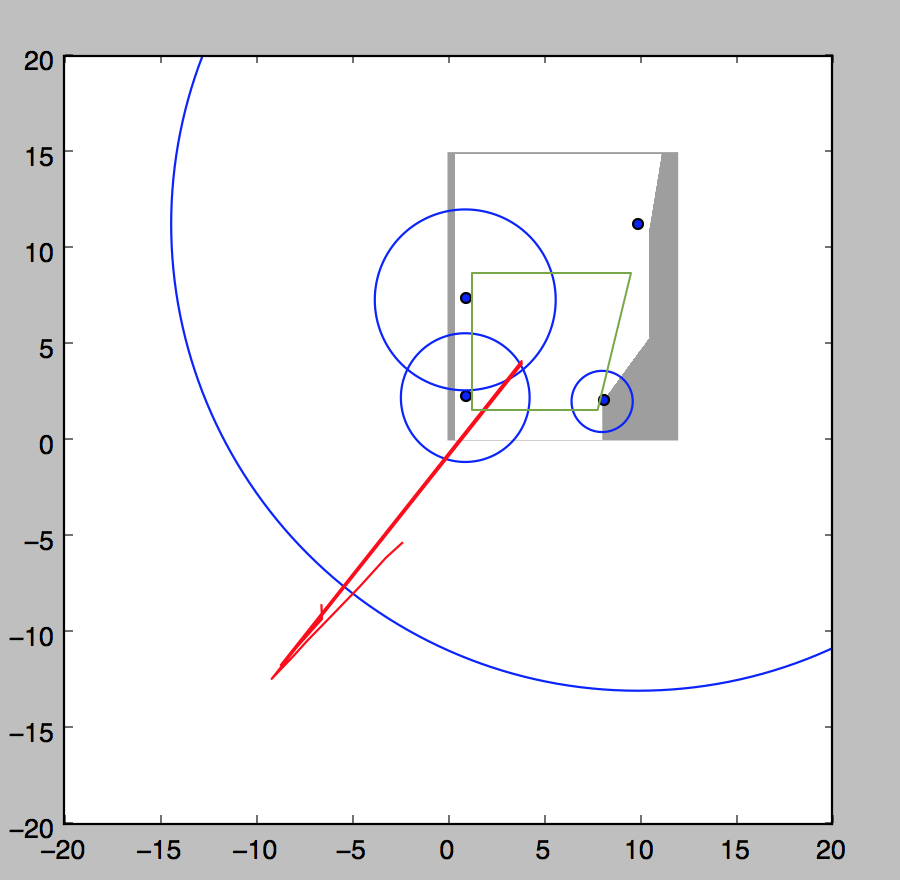
\includegraphics[width=0.45\textwidth]{figures/multilat_1}
  \label{fig:beacon_eval_multilat_1}
}
\subfloat[]{
  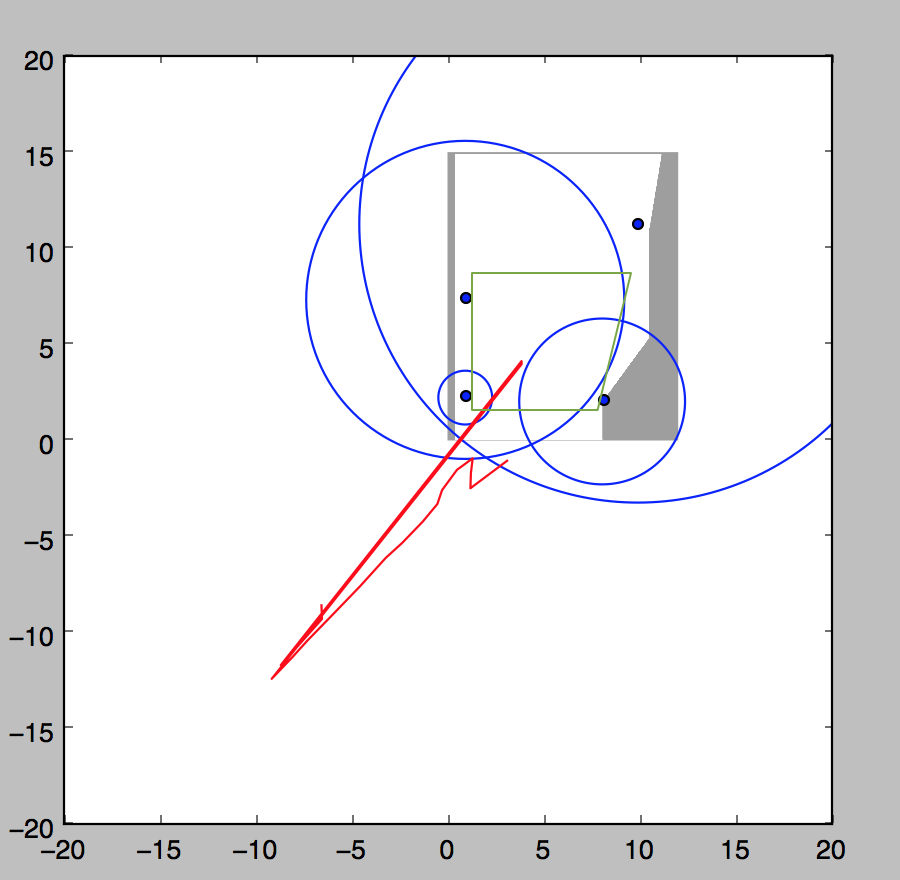
\includegraphics[width=0.45\textwidth]{figures/multilat_2}
}

\subfloat[]{
  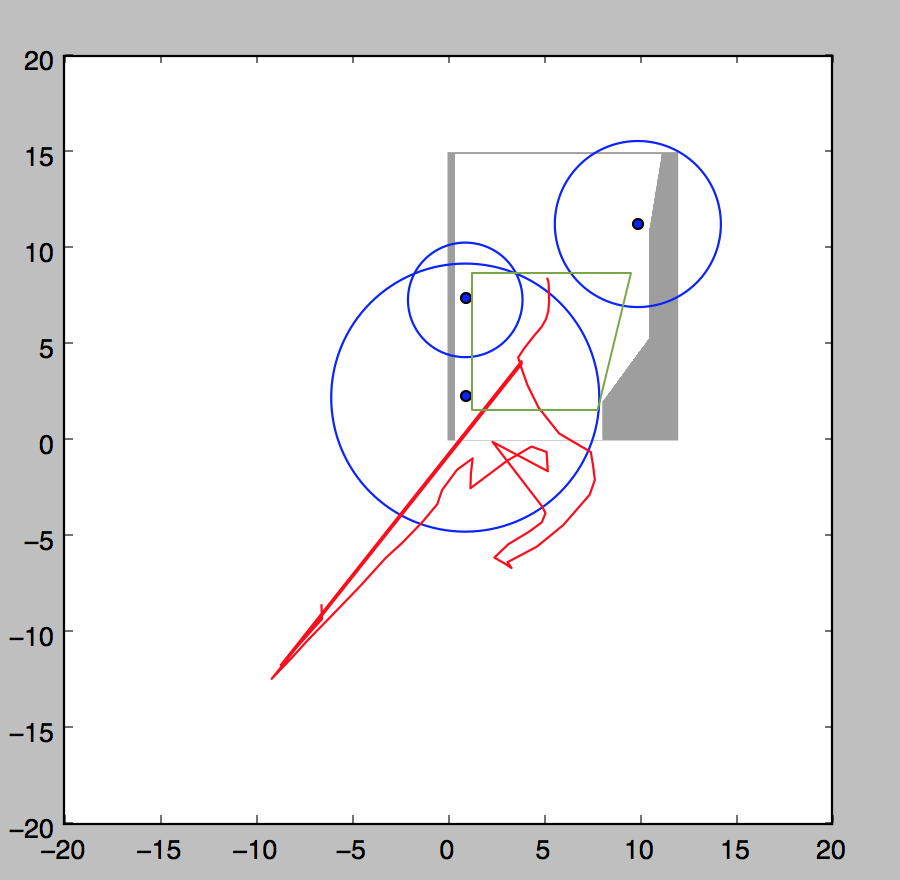
\includegraphics[width=0.45\textwidth]{figures/multilat_3}
  \label{fig:beacon_eval_multilat_3}
}
\subfloat[]{
  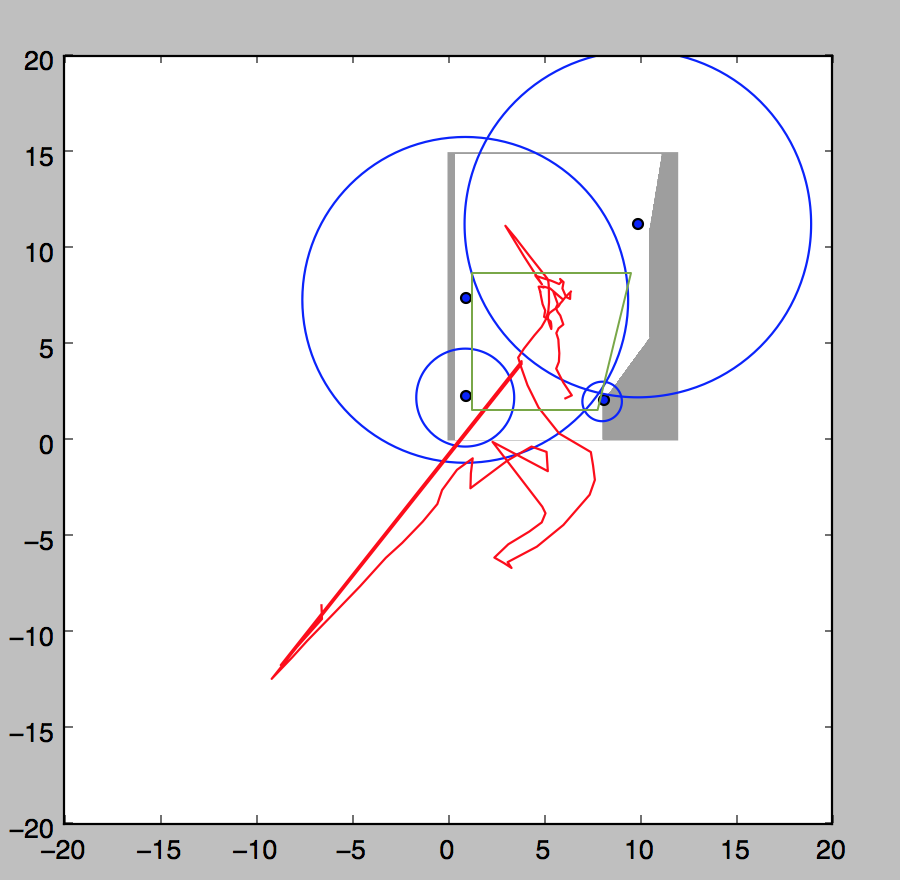
\includegraphics[width=0.45\textwidth]{figures/multilat_4}
}

  \caption{Four successive screenshots of the indoor self-localization experiment in a lecture hall (HTWG-KN F007) using multilateration. The screenshots show a map of the lecture hall, the walked path in green, the beacons as blue filled circles and their estimated distances as large blue circles. The red line depicts the estimated path.}
  \label{fig:beacon_eval_multilat}
\end{figure}

After evaluating the distance estimation's quality of one beacon, some beacons were deployed in a lecture hall to get a better feeling of how good the distance estimation actually works. On one hand, the goal was to visualize the estimated distances on a map to proof their plausibility, and on the other hand, to test if indoor self-localization with smartphones is possible by just using iBeacons without integrating additional sensor or map data.

As already mentioned in Section~\ref{sec:fund_trilateration}, \emph{multilateration} is a method to estimate a position by using the distances to several transmitters. If one uses only one sender then the receiver's position is somewhere on a circle around the transmitter with the estimated distance as radius of the circle.
By using two tranmitters $t_1$ and $t_2$, the two circles around the transmitters can have zero, one or two intersections, if the position of $t_1 \neq t_2$. Thus, the receiver's position must be at one of the circles' intersections.
By adding a third transmitter $t_3$ the three circles have either no or exactly one, common intersection point, which is the receiver's position. This applies also to more than three transmitters.

To be able to use the implementation with variable transmitter count the \emph{Least Square} method to determine the receiver's position was used. Another advantage is that the least square method can also estimate a position if no common intersection point exists.

For the experiment the same lecture hall as before was used. There, four beacons were positioned. Then the test device, which is an iPhone\,5S, was used to recorded the received beacon identifiers with their corresponding estimated distances, i.e.\ the \texttt{accuracy} values, provided by \acs{CL}, during a test walk on a defined path.
To visualize the estimated distances to the beacons and the user's estimated position, i.e.\ the walked path, a small Python program was used. Figure~\ref{fig:beacon_eval_multilat} shows four screenshots of the program's output. Each of it shows a map, which shows the lecture hall walls in grey. The white space in the hall is free space. The filled small blue circles next to the walls are the four beacons. The beacon is only shown if its signal was received during this time step. The big blue circles, are the circles around the beacons, where the radius represents the estimated distance to the beacons. The test person walked on the green tetragon, beginning at the bottom right corner in counter clockwise direction by holding the test device in front of oneself. The beacons were positioned at approximately the same height as the device in the test person's hand. The red line shows the estimated path.

\begin{figure}
	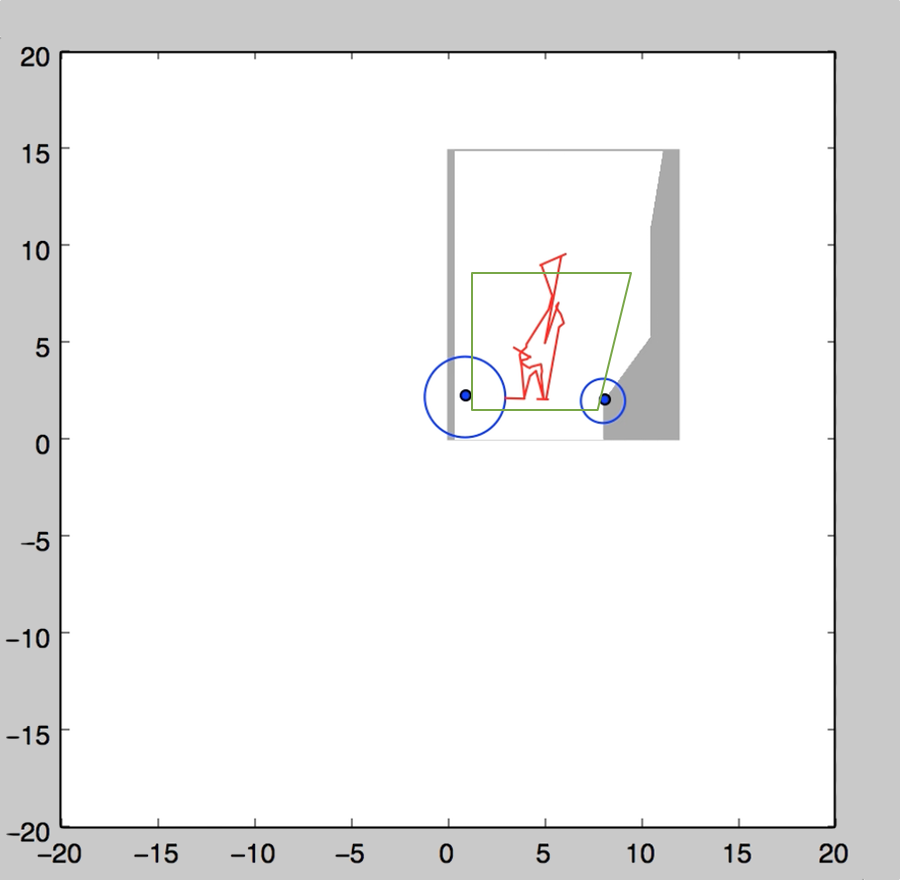
\includegraphics[width=0.45\textwidth]{figures/multilat_less5m}
	\caption{Screenshots of the indoor self-localization experiment in a lecture hall (HTWG-KN F007) using multilateration by only ignoring estimated distances more than 5\,m. The screenshots show a map of the lecture hall, the walked path in green, the beacons as blue filled circles and their estimated distances as large blue circles. The red line depicts the estimated path.}
	\label{fig:beacon_eval_multilat_less5m}
\end{figure}

The first screenshot depicted in Figure~\ref{fig:beacon_eval_multilat_1} shows, that the estimated distance sometimes is completely wrong, as shown by the blue circle around the top-right beacon. It also shows that the estimated position is somewhere several meters outside of the lecture hall. The second screenshot depicted in Figure~\ref{fig:beacon_eval_multilat_2}, shows, that the distance to the top-right beacon shrinks, but the one to the top-left massively grows. The distances to the other two beacons seem to be plausible. Figure~\ref{fig:beacon_eval_multilat_3} shows a plausible position. It also shows, that in this step the beacon's signal, positioned at the bottom-right corner, was not received. The last screenshot, depicted in Figure~\ref{fig:beacon_eval_multilat_4} shows also a more or less plausible position. The distances, except the one to the beacon, positioned at the bottom-left corner, seem to be plausible.

The experiment was repeated with the same setting and recorded data, but only used those beacon signals where the \texttt{accuracy} was $<$\,5\,m. Signals with larger estimated distances were ignored. Figure~\ref{fig:beacon_eval_multilat_less5m} shows the result. The estimated path actually is inside of the lecture hall. It is not possible to determine that the test person walked on the green path, but ignoring values more than 5\,m seems to improve the location estimation.

This experiment shows, that due to the very unreliable distance estimations the beacons' signals must be heavily influenced. It also shows that pure multilateration, without filtering the data and without integrating additional data sources, is not sufficient for indoor self-localization.

\subsection{Summary}
The results show, that the distance estimation not just depend on the beacons calibration, it also depends on the buildings construction form, the phones relative orientation to the beacons, and the obstacles in between.

It also points out, that the \texttt{CLBeacon}'s \texttt{accuracy} i.e.\ the estimated distance, comes very close to the actual distance up to 4\,--\,5\,m with \acs{LOS}. Larger distances cause a much higher spreading and thus, a larger error. Physical material like humans and walls cause attenuation, which results in a larger distance estimation than it actually is. Besides that, the estimated distance is sometimes very small compared to the actual distance.

To conclude, the estimated distances are very unreliable. Thus, their plausibility should be proven to filter the measurements. But due to the fact, that the validity cannot be proven without knowing the exact position of the receiver and the properties of all other influencing factors, which is not a trivial problem in large buildings, the only one possible improvement that could be applied, is to ignore beacons with an estimated distance larger than 5\,m. This solves of course not the problem with those beacons, which appear to be closer than they actually are. But from my point of view no real solution exists to solve this problem.